\documentclass[aspectratio=169]{beamer}
\usetheme{Luebeck}
%\usecolortheme{seahorse}
\useinnertheme{rectangles}
\useoutertheme{infolines}
\usepackage{xcolor}
\usepackage[utf8]{inputenc}
\usepackage{tikz}
\usepackage{tabularx}
\usepackage{lipsum}
\usepackage{amsmath,graphicx,dsfont}
\usetikzlibrary{shapes,backgrounds,arrows,automata,snakes,shadows,positioning, mindmap}
%===================================
\newcommand{\backupbegin}{
   \newcounter{framenumberappendix}
   \setcounter{framenumberappendix}{\value{framenumber}}
}
\newcommand{\backupend}{
   \addtocounter{framenumberappendix}{-\value{framenumber}}
   \addtocounter{framenumber}{\value{framenumberappendix}} 
}

\makeatletter
\setbeamertemplate{footline}
{
  \leavevmode%
  \hbox{%
  \begin{beamercolorbox}[wd=.333333\paperwidth,ht=2.25ex,dp=1ex,center]{author in head/foot}%
    \usebeamerfont{author in head/foot}\insertshortauthor%~~\beamer@ifempty{\insertshortinstitute}{}{(\insertshortinstitute)}
  \end{beamercolorbox}%
  \begin{beamercolorbox}[wd=.333333\paperwidth,ht=2.25ex,dp=1ex,center]{title in head/foot}%
    \usebeamerfont{title in head/foot}\insertshorttitle
  \end{beamercolorbox}%
  \begin{beamercolorbox}[wd=.333333\paperwidth,ht=2.25ex,dp=1ex,right]{date in head/foot}%
    \usebeamerfont{date in head/foot}\insertshortdate{}\hspace*{2em}
    \insertframenumber{} / \inserttotalframenumber\hspace*{2ex} 
  \end{beamercolorbox}}%
  \vskip0pt%
}
\makeatother
%===================================
\definecolor{Framableu}{RGB}{12,91,122}
\definecolor{Framableulight}{RGB}{18,144,176}
\definecolor{Nicered}{RGB}{176,18,65}
%\definecolor{Nicered}{RGB}{141,14,52}
\definecolor{Lightpink}{RGB}{229,177,218}
\definecolor{Green}{RGB}{144,176,18}
\definecolor{Lightcomplement}{RGB}{235,204,196}
\definecolor{Darkgoldenrod}{RGB}{176,144,18}
\definecolor{Darkomplement}{RGB}{122,43,12}
\definecolor{Complement}{RGB}{176,50,18}
\definecolor{Darkgreen}{RGB}{52,141,14}
%===================================
\setbeamertemplate{itemize items}[square]
\setbeamertemplate{blocks}[shadow=false]
\setbeamertemplate{caption}{\raggedright\insertcaption\par}
%===================================
\setbeamercolor{section in head/foot}{fg=white,bg=Framableu}
\setbeamercolor{subsection in head/foot}{fg=white,bg=Framableulight}
\setbeamercolor{author in head/foot}{bg=Framableu}
\setbeamercolor{item}{fg=Framableulight}
\setbeamercolor*{structure}{bg=Framableulight!20,fg=Framableulight}
\setbeamercolor*{palette secondary}{use=structure,fg=white,bg=structure.fg!75}
\setbeamercolor{section in toc}{fg=Framableu,bg=white}
\setbeamercolor{frametitle}{fg=Framableu!80,bg=white}
\setbeamercolor{block title}{fg=white, bg=Framableulight}  
%===================================
\title{Mixture tree model for network inference}
 \subtitle{Supervision:  S. Robin$^{\inst{1}}$ et C. Ambroise$^{\inst{1}\inst{2}$ }}
\author{Raphaëlle Momal} 
\institute[]
{
  \inst{1}%
  UMR AgroParisTech / INRA MIA-Paris \\
  \inst{2}%
  LaMME, Evry
  }
\date{July 7, 2018}

\newcommand{\Ccal}{\mathcal{C}}
\newcommand{\edgeunit}{1.5}
\newcommand{\emphase}[1]{\textcolor{Complement}{#1}}
\newcommand{\bleu}[1]{\textcolor{Framableulight}{#1}}
\newcommand{\pos}[1]{\textcolor{Darkgreen}{#1}}
\newcommand{\nega}[1]{\textcolor{Nicered}{#1}}
\newcommand\independent{\protect\mathpalette{\protect\independenT}{\perp}}\def\independenT#1#2{\mathrel{\rlap{$#1#2$}\mkern2mu{#1#2}}}
\newcommand{\Ncal}{\mathcal{N}}
\tikzset{%
    observed/.style={%
    scale=0.6,circle,draw=Framableulight,transform shape,fill=white,font=\Large}
}
\newcommand{\argmax}{\mathop{\mathrm{argmax}}}   
%#################################################################
\usepackage{graphicx}
\begin{document}
%\AtBeginSection[]{
%   \begin{frame}
   %%% affiche en début de chaque section, les noms de sections et
   %%% noms de sous-sections de la section en cours.
%   \tableofcontents[currentsection,hideothersubsections]
%   \end{frame} 
%}
\frame{\titlepage}


\section{Motivation}
%====================================================================
%====================================================================

\begin{frame}{Context}

Rising interest in \emphase{jointly analysed }species abundances:
\begin{itemize}
	\item Metagenomics 
	\item Microbiology
	\item Ecology
\end{itemize}
%\pause

\begin{block}{Ecological network}
Tool to better understand species interactions (direct/indirect), eco-systems organizations (clusters ?) 
\end{block}\bigskip
%\pause
Allows for resilience analyses, pathogens control, ecosystem comparison, response prediction...
\end{frame}
%====================================================================
%====================================================================


\begin{frame}{Data example}
	\begin{itemize}
	\item \emphase{Species}: bacteria, fungi...
	\item \emphase{Abundances}: read counts from Next-Generation Sequencing technologies (metabarcoding)
	\item \emphase{Covariates}: sequencing depth, temperature, water depth...  \bigskip
	
\end{itemize}
	Repeated signal : $n$ samples, $p$ abundances.
%\pause
\begin{block}{Data table}
	$Y = [Y_{ij}]_{(i,j) \in \{1,...,n\} \times \{1,..., p\}} $
	\begin{itemize}
	\item $Y_{ij}$: abundance of the $j^{th}$ species in the $i^{th}$ sample
\end{itemize}
\end{block}
\begin{center}
	Infer the \emphase{species interaction network} from count data $Y$
\end{center}
\end{frame}
%====================================================================
%====================================================================
\begin{frame}{Challenges}\large{
	\begin{itemize}
	\item  Statistical network inference \bigskip\bigskip
	\item Count data \bigskip\bigskip
	\item Offsets and covariates
\end{itemize}}
\end{frame}
%====================================================================
%====================================================================

\section{Network inference}
\subsection{General Framework}
%====================================================================
%===================================================================

\begin{frame}{Graphical models: a statistical framework for network inference}
\bleu{Example}:\bigskip
\begin{columns}
\begin{column}{0.3\linewidth}\hspace{0.5cm}
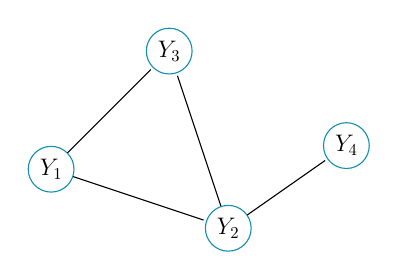
\begin{tikzpicture}	

      \tikzstyle{every edge}=[-,>=stealth',shorten >=1pt,auto,thin,draw]
		\node[observed] (Y1) at (0*\edgeunit, 0*\edgeunit) {$Y_1$};
		\node[observed] (Y2) at (1.5*\edgeunit, -0.5*\edgeunit) {$Y_2$};
		\node[observed] (Y3) at (1*\edgeunit, 1*\edgeunit) {$Y_3$};
		\node[observed] (Y4) at (2.5*\edgeunit, 0.2*\edgeunit) {$Y_4$};
		\path (Y1) edge [] (Y2)
        (Y1) edge [] (Y3)
        (Y2) edge [] (Y3)
        (Y2) edge [] (Y4);
	\end{tikzpicture}\\
\end{column}
\begin{column}{0.5\linewidth}
	\begin{itemize}
	\item All variables are dependant \bigskip
	\item Some are \emphase{conditionally independent} (i.e. indirectly dependeant)\\\bigskip
	 $Y_4$ is independent from $(Y_1, Y_3)$ conditionally on $Y_2$
\end{itemize}
\end{column}
\end{columns}

\end{frame}
%====================================================================
%====================================================================

\begin{frame}{Graphical models}
\begin{block}{Definition \cite{Lau96}}
	The joint distribution P is faithful to the graph G iff \[ P(Y_1, \dots, Y_p) \propto \prod_{C \in \Ccal_G} \psi_C(Y_C) \]
  where $\Ccal_G =$ set of maximal cliques of $G$.
\end{block}
%\pause
\begin{columns}
\begin{column}{0.4\linewidth}
\flushright
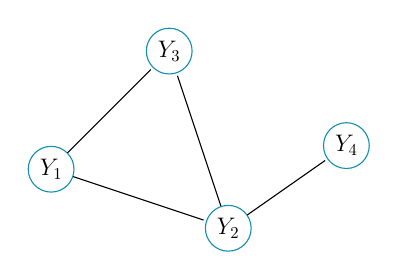
\begin{tikzpicture}	

      \tikzstyle{every edge}=[-,>=stealth',shorten >=1pt,auto,thin,draw]
		\node[observed] (Y1) at (0*\edgeunit, 0*\edgeunit) {$Y_1$};
		\node[observed] (Y2) at (1.5*\edgeunit, -0.5*\edgeunit) {$Y_2$};
		\node[observed] (Y3) at (1*\edgeunit, 1*\edgeunit) {$Y_3$};
		\node[observed] (Y4) at (2.5*\edgeunit, 0.2*\edgeunit) {$Y_4$};
		\path (Y1) edge [] (Y2)
        (Y1) edge [] (Y3)
        (Y2) edge [] (Y3)
        (Y2) edge [] (Y4);
	\end{tikzpicture}\\
\end{column}
\begin{column}{0.6\linewidth}
\begin{align*}
	P(Y_1, &Y_2, Y_3, Y_4) \propto \\ 
	& \psi_1(Y_1 ,Y_2, Y_3) \times \psi_2(Y_3, Y_4)
\end{align*} 
\end{column}
\end{columns}
\end{frame}

\subsection{Using trees}
%====================================================================
%====================================================================

\begin{frame}{Spanning trees}
	Unconstrained graph $\Rightarrow$ very large space to explore: \emphase{$\text{\#} \mathcal{G}_p = 2^{\frac{p(p-1)}{2}}$}\\ \bigskip
	
	Spanning trees are a \bleu{sparse} solution :
	$$
  \left. \begin{tabular}{l}
          $G$ is connected \\
          $G$ has no cycle
         \end{tabular} \right\}
  \text{ $G$ has $(p-1)$ edges}
  $$
  \begin{columns}
  \begin{column}{6cm}
	\begin{figure}[htp]
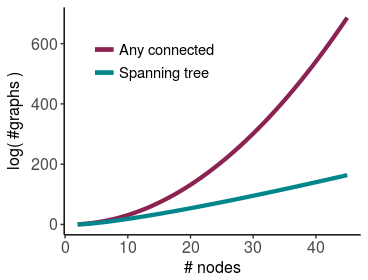
\includegraphics[width=5cm]{compar_typegraphs.png}
	\end{figure}
	\end{column}
	 \begin{column}{6cm}
Much \bleu{ smaller space} to explore:\\  \emphase{$$\text{\#} \mathcal{T}_p = p^{(p-2)}$$}\\ \bigskip
\pause
Still a huge complexity...
\end{column}
\end{columns}
\end{frame}
%====================================================================
%====================================================================
\begin{frame}{Maximizing and summing over spanning trees}
\begin{description}
\item[Maximum spanning tree] Kruskall's algorithm\\
 $$ \hat{T} = \underset{T}{\mathrm{argmax }} \left\{\prod_{(k,l) \in T} \psi_{k,l}(Y) \right\}  \rightarrow \emphase{\Theta (p^2)}$$ \bigskip 
\item[Tree averaging] Matrix tree theorem \cite{matrixtree}\\ 
$$ \sum_T\prod_{(k,l) \in T} \psi_{k,l}(Y) = \det(L(Y))  \rightarrow \emphase{\Theta (p^3)}$$
\end{description}\pause \bigskip 
\center{
\textbf{Approach}: infer the network by \emphase{averaging spanning trees}}
	
\end{frame}
%====================================================================
%====================================================================

\begin{frame}{Tree averaging} 
\begin{center}
    

%\begin{tabular}{p{\linewidth}}
%\begin{tabularx}{\linewidth}{ccccl}
 \begin{tabular}{ccccl}
   \begin{tabular}{c}
	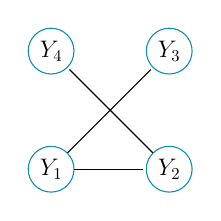
\begin{tikzpicture}
		
      \tikzstyle{every edge}=[-,>=stealth',shorten >=1pt,auto,thin,draw]
    
		\node[observed] (Y1) at (0*\edgeunit, 0*\edgeunit) {$Y_1$};
		\node[observed] (Y2) at (1*\edgeunit, 0*\edgeunit) {$Y_2$};
		\node[observed] (Y3) at (1*\edgeunit, 1*\edgeunit) {$Y_3$};
		\node[observed] (Y4) at (0*\edgeunit, 1*\edgeunit) {$Y_4$};
		\path (Y1) edge [] (Y2)
        (Y1) edge [] (Y3)
        (Y2) edge [] (Y4);
   
	\end{tikzpicture}\\
	\footnotesize{$P\{T = T_1 | Y\}$}
	   \end{tabular}
	   & 
	 %  \hspace{-.05\textwidth}% \pause
	   \begin{tabular}{c}
		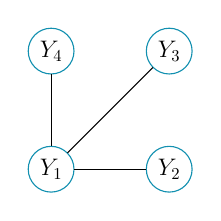
\begin{tikzpicture}
		\tikzstyle{every observed}=[draw=none,text=black,scale=0.5,
      transform shape,circular drop shadow] 
		\node[observed] (Y1) at (0*\edgeunit, 0*\edgeunit) {$Y_1$};
		\node[observed] (Y2) at (1*\edgeunit, 0*\edgeunit) {$Y_2$};
		\node[observed] (Y3) at (1*\edgeunit, 1*\edgeunit) {$Y_3$};
		\node[observed] (Y4) at (0*\edgeunit, 1*\edgeunit) {$Y_4$};
		
		\path (Y1) edge [] (Y2)
        (Y1) edge [] (Y3)
        (Y1) edge [] (Y4);
		\end{tikzpicture} \\
		\footnotesize{$P\{T = T_2 | Y\}$}
	   \end{tabular}
	   &
	  % \hspace{-.05\textwidth} %\pause
	   \begin{tabular}{c}
		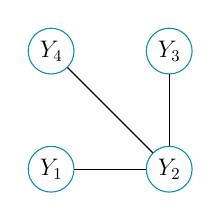
\begin{tikzpicture}
		\tikzstyle{every observed}=[draw=none,text=black,scale=0.5,
      transform shape,circular drop shadow] 
		\node[observed] (Y1) at (0*\edgeunit, 0*\edgeunit) {$Y_1$};
		\node[observed] (Y2) at (1*\edgeunit, 0*\edgeunit) {$Y_2$};
		\node[observed] (Y3) at (1*\edgeunit, 1*\edgeunit) {$Y_3$};
		\node[observed] (Y4) at (0*\edgeunit, 1*\edgeunit) {$Y_4$};
		
		\path (Y1) edge [] (Y2)
        (Y2) edge [] (Y3)
        (Y2) edge [] (Y4); 
		\end{tikzpicture}\\
		\footnotesize{$P\{T = T_3 | Y\}$}
	   \end{tabular}
	   &
	  % \hspace{-.05\textwidth}% \pause
	   \begin{tabular}{c}
		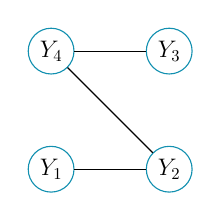
\begin{tikzpicture}
		\tikzstyle{every observed}=[draw=none,text=black,scale=0.5,
      transform shape,circular drop shadow] 
		\node[observed] (Y1) at (0*\edgeunit, 0*\edgeunit) {$Y_1$};
		\node[observed] (Y2) at (1*\edgeunit, 0*\edgeunit) {$Y_2$};
		\node[observed] (Y3) at (1*\edgeunit, 1*\edgeunit) {$Y_3$};
		\node[observed] (Y4) at (0*\edgeunit, 1*\edgeunit) {$Y_4$};
		 
		\path (Y1) edge [] (Y2)
        (Y3) edge [] (Y4)
        (Y2) edge [] (Y4);
		\end{tikzpicture} \\
		\footnotesize{$P\{T = T_4 | Y\}$}
	   \end{tabular}
	   & %\hspace{-.06\textwidth} 
	   \huge{\emphase{...}}\normalsize   \\ \\
	   \\% \pause
	   \begin{tabular}{l}
		Compute edge\\
		probabilities:
	   \end{tabular}
	   &
	  % \hspace{-.05\textwidth}
	   \begin{tabular}{c}
		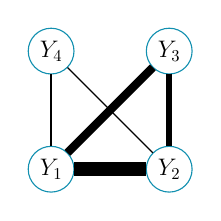
\begin{tikzpicture}
		\node[observed] (Y1) at (0*\edgeunit, 0*\edgeunit) {$Y_1$};
		\node[observed] (Y2) at (1*\edgeunit, 0*\edgeunit) {$Y_2$};
		\node[observed] (Y3) at (1*\edgeunit, 1*\edgeunit) {$Y_3$};
		\node[observed] (Y4) at (0*\edgeunit, 1*\edgeunit) {$Y_4$};
		\draw [line width=5pt] (Y1) -- (Y2); 
		\draw [line width=3pt] (Y1) -- (Y3); 
		\draw [line width=.5pt] (Y1) -- (Y4); 
		\draw [line width=2pt] (Y2) -- (Y3); 
		\draw [line width=.5pt] (Y2) -- (Y4); 
 %		\draw [line width=.5pt] (Y3) -- (Y4); 
		\end{tikzpicture}\\
		\emphase{$P\{(j, k) \in T | Y\}$}
	   \end{tabular}
	   &
	  % \hspace{-.05\textwidth} %\pause
	   \begin{tabular}{l}
		Thresholding\\
		probabilities:
	   \end{tabular}
	   &
	   %\hspace{-.05\textwidth}
	   \begin{tabular}{c}
		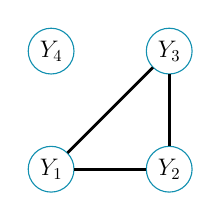
\begin{tikzpicture}
		\node[observed] (Y1) at (0*\edgeunit, 0*\edgeunit) {$Y_1$};
		\node[observed] (Y2) at (1*\edgeunit, 0*\edgeunit) {$Y_2$};
		\node[observed] (Y3) at (1*\edgeunit, 1*\edgeunit) {$Y_3$};
		\node[observed] (Y4) at (0*\edgeunit, 1*\edgeunit) {$Y_4$};
		\draw [line width=1pt] (Y1) -- (Y2); 
		\draw [line width=1pt] (Y1) -- (Y3); 
% 		\draw [line width=1pt] (Y1) -- (Y4); 
		\draw [line width=1pt] (Y2) -- (Y3); 
% 		\draw [line width=.1pt] (Y2) -- (Y4); 
% 		\draw [line width=1pt] (Y3) -- (Y4); 
		\end{tikzpicture}\\
		\emphase{$P\{(j, k) \in T | Y\}$}
	   \end{tabular}
	   &
	 \end{tabular}
   % \end{tabular}
   %\end{tabularx}
   \end{center}
\end{frame}
%====================================================================
%====================================================================


\section{With count data}
\subsection{Model}

%====================================================================
%====================================================================

\begin{frame}{PLN model}
\begin{block}{Poisson log-Normal distribution \cite{AiH89}}
\[
            \left.
                \begin{array}{rl}
               \vspace{0.2cm}    Z_i \textit{ iid } &\sim \mathcal{N}_{d}(0,\Sigma)\\
              \vspace{0.2cm}    &(Y_{ij})_j \independent |Z_i\\
                    Y_{ij}|Z_{ij} &\sim \mathcal{P}(e^{\only<2-3>{\emphase{o_{ij}+x_i^{\text{T}}\Theta_j} +}Z_{ij}}) 
                   
                \end{array}
            \right \} Y \sim \mathcal{PLN}(\only<2-3>{\emphase{O+x^{\text{T}}\Theta }}\only<1>{0}, \Sigma)  
            \]
\end{block}

\begin{itemize}
    \item Dependency structure in the Gaussian latent layer
    \item Easy handling of multi-variate data (contrary to Negative binomial distribution)
  \only<2->{ \item Allow adjustment for covariates and offsets}
  \only<3>{\item Variational estimation algorithm \cite{CMR17}}
\end{itemize}
%\pause
\only<3>{\center{ \textbf{ Approach:} Infer the \emphase{latent Gaussian network} with an \emphase{VEM algorithm.}}}
\end{frame}

%====================================================================
%====================================================================
\section{Simulation}
\subsection{Competitor}
%====================================================================
%====================================================================

\begin{frame}{Gaussian Graphical Models (GGM) }
   \emphase{Gaussian distribution:}\\
 \begin{center}
	$  Y_i \sim \Ncal_p(\mu, \Sigma) $, $\mu =$ vector of means, $\Sigma =$ covariance matrix.
 % \[L(Y,\Omega) \propto \frac{n}{2}\log(det(\Omega))-\frac{n}{2} Y^T\Omega Y\]
\end{center}
  
 
  
   \bigskip %\pause
  \emphase{A nice property:} ~ \\

  \begin{columns}
  \begin{column}{0.15\textwidth}
	
\end{column}
  \begin{column}{0.4\textwidth}
   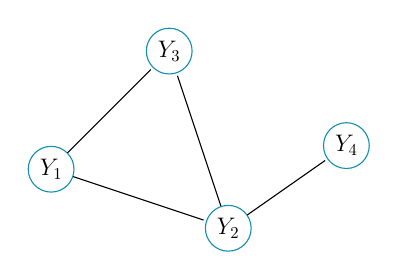
\begin{tikzpicture}	

       \tikzstyle{every edge}=[-,>=stealth',shorten >=1pt,auto,thin,draw]
		\node[observed] (Y1) at (0*\edgeunit, 0*\edgeunit) {$Y_1$};
		\node[observed] (Y2) at (1.5*\edgeunit, -0.5*\edgeunit) {$Y_2$};
		\node[observed] (Y3) at (1*\edgeunit, 1*\edgeunit) {$Y_3$};
		\node[observed] (Y4) at (2.5*\edgeunit, 0.2*\edgeunit) {$Y_4$};
		\path (Y1) edge [] (Y2)
        (Y1) edge [] (Y3)
        (Y2) edge [] (Y3)
        (Y2) edge [] (Y4);
	\end{tikzpicture}
    \end{column}
    \begin{column}{8cm}
 
    \begin{tabular}{p{.5\textwidth}}
	 Inverse covariance matrix
	 $$
	 \Sigma^{-1} = \Omega \propto \left[ \begin{array}{cccc}
	   1 & .5 & .5 & \emphase{0} \\
	   .5 & 1 & .5 & .5 \\
	   .5 & .5 & 1 & \emphase{0} \\
	   \emphase{0} & .5& \emphase{0}  & 1
	   \end{array} \right] 
	 $$
    \end{tabular} 
   
  \end{column}
  \end{columns}
  \pause
 \emphase{Glasso on gaussian data:}\hspace{0.2cm} $\widehat{\Omega}_\lambda = \arg\min_{\Omega \in \mathcal{S}_d^+}\left\{ L(Y,\Omega)+\lambda \sum_{i\neq j} |\omega_{ij}| \right\} \hspace{0.5cm} $\\
 \begin{center}
	$\Rightarrow$ {\color{Framableulight}SpiecEasi method \cite{kurtz}}: glasso on transformed counts
\end{center}

% $$
% \widehat{\Sigma} \propto \left[ \begin{array}{cccc}
%   1 & -.02 & -.49 & .25 \\
%   -.02 & 1 & -.62 & .36 \\
%   -.49 & -.62 & 1 & -.61 \\
%   .25 & .36 & -.61 & 1
%   \end{array} \right] 
% $$

\end{frame}
%====================================================================
%====================================================================

\subsection{}
%====================================================================
%====================================================================

\begin{frame}{Simulation design}

\begin{enumerate}
     \item Choose  \emphase{$G$} and define  \emphase{$\Omega$} accordingly\vspace{0.3cm} 
     \item Sample count data \emphase{$Y$} from $\mathcal{PLN}(0,\Omega^{-1})$ with possible covariates
     \item Infer the network with \emphase{PLN + mixture tree VEM}  and \emphase{SpiecEasi} \vspace{0.3cm}
     \item Compare results with \emphase{AUC} (presence/absence of edges)
\end{enumerate}\bigskip\bigskip
\hspace{1cm}$\Rightarrow$ 40 replicates for each setting $(p, n, \text{edge probability})$
	
\end{frame}
%====================================================================
%====================================================================

\begin{frame}{Results: Erdös, 20 nodes}
\begin{figure}[htp]
\centering
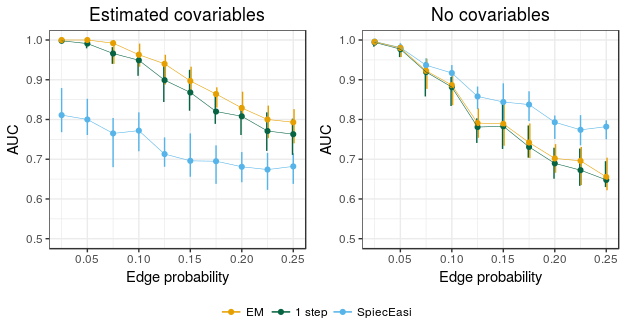
\includegraphics[width=13cm]{mosaic.png}
\end{figure}
\end{frame}


%====================================================================
%====================================================================
\section{Application}
\subsection{Oak data}

%====================================================================
%====================================================================

\begin{frame}{Oak Mildew}
\begin{columns}
\begin{column}{5cm}
\begin{figure}[htp]
\centering
\includegraphics[scale=0.07]{EA.jpg}
\caption{\textit{Pathogen Erysiphe alphitoides (EA).}}
\end{figure}
\end{column}
\begin{column}{6cm}
\begin{figure}[htp]
\centering
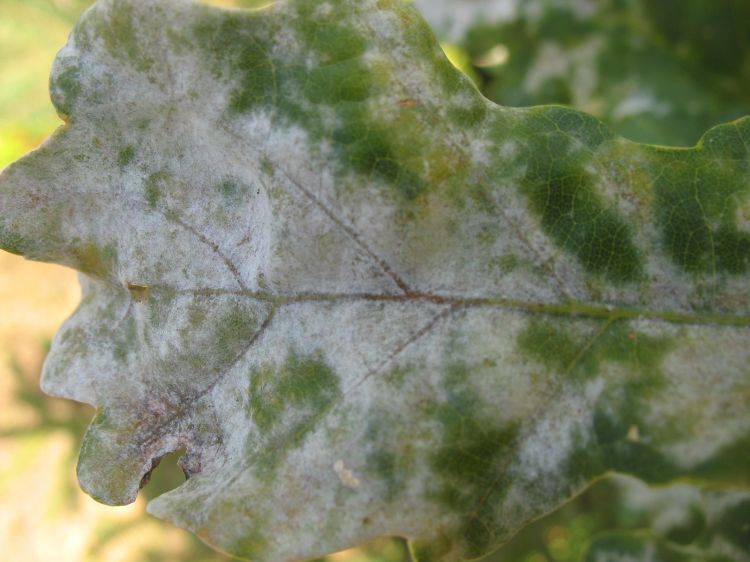
\includegraphics[scale=0.1]{mildew.jpg}
\caption{Oak leaf with powdery mildew.}
\end{figure}
\end{column}
\end{columns}
\vspace{0.5cm}
Metabarcoding of oak tree leaves microbiome \cite{jakuch}.\\

\begin{itemize}
	\item 114 sample of 94 microbial species counts (bacteria/fungi)
	\item Different read depth for bacteria and fungi: unsuited for normalization with SpiecEasi
	\item 3 quantitative covariates 
\end{itemize}\bigskip
We are interested in EA and F19, a second major fungi.
\end{frame}
%====================================================================
%====================================================================


\begin{frame}{Model with covariates}
	\begin{description}
	\item[Regression coefficients]\begin{itemize}
	\item []
\end{itemize}% \begin{table}[]
%\begin{tabular}{l|lllll}
%    & Offset & \multicolumn{4}{|c}{Adding distances}   \\\cline{2-6}
%    & \multicolumn{1}{l|}{Int.}  & Int.  & to base & to trunk & to ground \\\hline
%EA  & \nega{-4.39}  &\pos{ 0.710 }&  \nega{-0.0200} &\pos{ 0.0215  } &  \nega{-0.0251  } \\
%F19 &  \nega{-4.37}  &  \nega{-8.52} & \pos{0.0219 } &  \nega{-0.0172}  & \pos{0.0143  } 
%\end{tabular}
%\end{table}

\begin{table}[]
\begin{tabular}{l|lll}
  & \multicolumn{3}{|c}{Covariates $(\times 10^{-2})$}   \\\cline{2-4}
   .  & to base & to trunk & to ground \\\hline
EA  &  \nega{-2.00} &\pos{ 2.15  } &  \nega{-2.51  } \\
F19 & \pos{2.19 } &  \nega{-1.72}  & \pos{1.43  } 
\end{tabular}
\end{table}

	\item[Degree estimation]\begin{itemize}
	\item []
\end{itemize} \begin{table}[]
\begin{tabular}{l|ll}
    & Offset & Distances \\\hline
EA  & 2.20   & 1.86      \\
F19 & 3.03   & 2.80     
\end{tabular}
\end{table}
\end{description}
\end{frame}
%====================================================================
%====================================================================
\begin{frame}{Inferred networks}
\begin{figure}[htp]
\centering
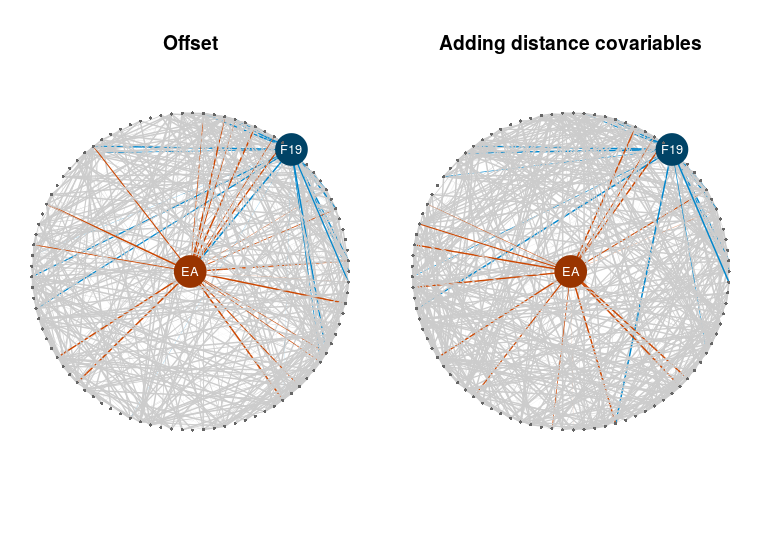
\includegraphics[width=11cm]{compare_reseaux.png}

\end{figure}

\end{frame}
%-----------------------------
%---------------------------
\begin{frame}{Conclusion}
\begin{description}
\item[Contributions:] 
\begin{itemize}
\item[]  
	\item Formal probabilistic model for network inference with \emphase{count data}
	\item  EM Estimation algorithm
	\item Inclusion of \emphase{offsets} and \emphase{covariates}
\end{itemize}
\bigskip 
\item[Perspectives:]

\begin{itemize}
\item[]  
	\item Method for determining the threshold
	\item Network comparison
	\item Model for the inference in the observed counts layer
	\item Missing major actor (species/covariable)
\end{itemize}
\end{description}
\end{frame}
%====================================================================
%====================================================================


\begin{frame}{Acknowledgments}

Special thanks :\\
\begin{description}
\item[Supervisors] Stéphane Robin, Christophe Ambroise
\item[PLN team] Julien Chiquet (MIA-Paris), Mahendra Mariadassou (INRA Jouy)
\item[Data] Corinne Vacher (INRA Bordeaux)
\end{description}
Contact :\\
\begin{description}
\item[email] raphaelle.momal@agroparistech.fr
\item[Web]Rmomal.github.io\\
\end{description}
\begin{center}
	
\includegraphics[width=0.25\linewidth]{logo_inra.jpg}\hspace{0.1cm}
	
\includegraphics[width=0.25\linewidth]{agro.PNG}
	
\includegraphics[width=0.25\linewidth]{lmh.png}\hspace{0.1cm}
	
\includegraphics[width=0.15\linewidth]{upsud.jpg}
    
\end{center}

\end{frame}
\appendix
\backupbegin
\begin{frame}[allowframebreaks]
\bibliographystyle{apalike}
{\footnotesize 
    \bibliography{biblio3.bib}}
\frametitle{References}
%\bibliography{cellcite}
\end{frame}\backupend
%====================================================================
%====================================================================

\end{document}